% Options for packages loaded elsewhere
\PassOptionsToPackage{unicode}{hyperref}
\PassOptionsToPackage{hyphens}{url}
\PassOptionsToPackage{dvipsnames,svgnames,x11names}{xcolor}
%
\documentclass[
  letterpaper,
  DIV=11,
  numbers=noendperiod]{scrartcl}

\usepackage{amsmath,amssymb}
\usepackage{iftex}
\ifPDFTeX
  \usepackage[T1]{fontenc}
  \usepackage[utf8]{inputenc}
  \usepackage{textcomp} % provide euro and other symbols
\else % if luatex or xetex
  \usepackage{unicode-math}
  \defaultfontfeatures{Scale=MatchLowercase}
  \defaultfontfeatures[\rmfamily]{Ligatures=TeX,Scale=1}
\fi
\usepackage{lmodern}
\ifPDFTeX\else  
    % xetex/luatex font selection
\fi
% Use upquote if available, for straight quotes in verbatim environments
\IfFileExists{upquote.sty}{\usepackage{upquote}}{}
\IfFileExists{microtype.sty}{% use microtype if available
  \usepackage[]{microtype}
  \UseMicrotypeSet[protrusion]{basicmath} % disable protrusion for tt fonts
}{}
\makeatletter
\@ifundefined{KOMAClassName}{% if non-KOMA class
  \IfFileExists{parskip.sty}{%
    \usepackage{parskip}
  }{% else
    \setlength{\parindent}{0pt}
    \setlength{\parskip}{6pt plus 2pt minus 1pt}}
}{% if KOMA class
  \KOMAoptions{parskip=half}}
\makeatother
\usepackage{xcolor}
\setlength{\emergencystretch}{3em} % prevent overfull lines
\setcounter{secnumdepth}{-\maxdimen} % remove section numbering
% Make \paragraph and \subparagraph free-standing
\makeatletter
\ifx\paragraph\undefined\else
  \let\oldparagraph\paragraph
  \renewcommand{\paragraph}{
    \@ifstar
      \xxxParagraphStar
      \xxxParagraphNoStar
  }
  \newcommand{\xxxParagraphStar}[1]{\oldparagraph*{#1}\mbox{}}
  \newcommand{\xxxParagraphNoStar}[1]{\oldparagraph{#1}\mbox{}}
\fi
\ifx\subparagraph\undefined\else
  \let\oldsubparagraph\subparagraph
  \renewcommand{\subparagraph}{
    \@ifstar
      \xxxSubParagraphStar
      \xxxSubParagraphNoStar
  }
  \newcommand{\xxxSubParagraphStar}[1]{\oldsubparagraph*{#1}\mbox{}}
  \newcommand{\xxxSubParagraphNoStar}[1]{\oldsubparagraph{#1}\mbox{}}
\fi
\makeatother

\usepackage{color}
\usepackage{fancyvrb}
\newcommand{\VerbBar}{|}
\newcommand{\VERB}{\Verb[commandchars=\\\{\}]}
\DefineVerbatimEnvironment{Highlighting}{Verbatim}{commandchars=\\\{\}}
% Add ',fontsize=\small' for more characters per line
\usepackage{framed}
\definecolor{shadecolor}{RGB}{241,243,245}
\newenvironment{Shaded}{\begin{snugshade}}{\end{snugshade}}
\newcommand{\AlertTok}[1]{\textcolor[rgb]{0.68,0.00,0.00}{#1}}
\newcommand{\AnnotationTok}[1]{\textcolor[rgb]{0.37,0.37,0.37}{#1}}
\newcommand{\AttributeTok}[1]{\textcolor[rgb]{0.40,0.45,0.13}{#1}}
\newcommand{\BaseNTok}[1]{\textcolor[rgb]{0.68,0.00,0.00}{#1}}
\newcommand{\BuiltInTok}[1]{\textcolor[rgb]{0.00,0.23,0.31}{#1}}
\newcommand{\CharTok}[1]{\textcolor[rgb]{0.13,0.47,0.30}{#1}}
\newcommand{\CommentTok}[1]{\textcolor[rgb]{0.37,0.37,0.37}{#1}}
\newcommand{\CommentVarTok}[1]{\textcolor[rgb]{0.37,0.37,0.37}{\textit{#1}}}
\newcommand{\ConstantTok}[1]{\textcolor[rgb]{0.56,0.35,0.01}{#1}}
\newcommand{\ControlFlowTok}[1]{\textcolor[rgb]{0.00,0.23,0.31}{\textbf{#1}}}
\newcommand{\DataTypeTok}[1]{\textcolor[rgb]{0.68,0.00,0.00}{#1}}
\newcommand{\DecValTok}[1]{\textcolor[rgb]{0.68,0.00,0.00}{#1}}
\newcommand{\DocumentationTok}[1]{\textcolor[rgb]{0.37,0.37,0.37}{\textit{#1}}}
\newcommand{\ErrorTok}[1]{\textcolor[rgb]{0.68,0.00,0.00}{#1}}
\newcommand{\ExtensionTok}[1]{\textcolor[rgb]{0.00,0.23,0.31}{#1}}
\newcommand{\FloatTok}[1]{\textcolor[rgb]{0.68,0.00,0.00}{#1}}
\newcommand{\FunctionTok}[1]{\textcolor[rgb]{0.28,0.35,0.67}{#1}}
\newcommand{\ImportTok}[1]{\textcolor[rgb]{0.00,0.46,0.62}{#1}}
\newcommand{\InformationTok}[1]{\textcolor[rgb]{0.37,0.37,0.37}{#1}}
\newcommand{\KeywordTok}[1]{\textcolor[rgb]{0.00,0.23,0.31}{\textbf{#1}}}
\newcommand{\NormalTok}[1]{\textcolor[rgb]{0.00,0.23,0.31}{#1}}
\newcommand{\OperatorTok}[1]{\textcolor[rgb]{0.37,0.37,0.37}{#1}}
\newcommand{\OtherTok}[1]{\textcolor[rgb]{0.00,0.23,0.31}{#1}}
\newcommand{\PreprocessorTok}[1]{\textcolor[rgb]{0.68,0.00,0.00}{#1}}
\newcommand{\RegionMarkerTok}[1]{\textcolor[rgb]{0.00,0.23,0.31}{#1}}
\newcommand{\SpecialCharTok}[1]{\textcolor[rgb]{0.37,0.37,0.37}{#1}}
\newcommand{\SpecialStringTok}[1]{\textcolor[rgb]{0.13,0.47,0.30}{#1}}
\newcommand{\StringTok}[1]{\textcolor[rgb]{0.13,0.47,0.30}{#1}}
\newcommand{\VariableTok}[1]{\textcolor[rgb]{0.07,0.07,0.07}{#1}}
\newcommand{\VerbatimStringTok}[1]{\textcolor[rgb]{0.13,0.47,0.30}{#1}}
\newcommand{\WarningTok}[1]{\textcolor[rgb]{0.37,0.37,0.37}{\textit{#1}}}

\providecommand{\tightlist}{%
  \setlength{\itemsep}{0pt}\setlength{\parskip}{0pt}}\usepackage{longtable,booktabs,array}
\usepackage{calc} % for calculating minipage widths
% Correct order of tables after \paragraph or \subparagraph
\usepackage{etoolbox}
\makeatletter
\patchcmd\longtable{\par}{\if@noskipsec\mbox{}\fi\par}{}{}
\makeatother
% Allow footnotes in longtable head/foot
\IfFileExists{footnotehyper.sty}{\usepackage{footnotehyper}}{\usepackage{footnote}}
\makesavenoteenv{longtable}
\usepackage{graphicx}
\makeatletter
\def\maxwidth{\ifdim\Gin@nat@width>\linewidth\linewidth\else\Gin@nat@width\fi}
\def\maxheight{\ifdim\Gin@nat@height>\textheight\textheight\else\Gin@nat@height\fi}
\makeatother
% Scale images if necessary, so that they will not overflow the page
% margins by default, and it is still possible to overwrite the defaults
% using explicit options in \includegraphics[width, height, ...]{}
\setkeys{Gin}{width=\maxwidth,height=\maxheight,keepaspectratio}
% Set default figure placement to htbp
\makeatletter
\def\fps@figure{htbp}
\makeatother

\usepackage{fvextra}
\DefineVerbatimEnvironment{Highlighting}{Verbatim}{breaklines,commandchars=\\\{\}}
\KOMAoption{captions}{tableheading}
\makeatletter
\@ifpackageloaded{caption}{}{\usepackage{caption}}
\AtBeginDocument{%
\ifdefined\contentsname
  \renewcommand*\contentsname{Table of contents}
\else
  \newcommand\contentsname{Table of contents}
\fi
\ifdefined\listfigurename
  \renewcommand*\listfigurename{List of Figures}
\else
  \newcommand\listfigurename{List of Figures}
\fi
\ifdefined\listtablename
  \renewcommand*\listtablename{List of Tables}
\else
  \newcommand\listtablename{List of Tables}
\fi
\ifdefined\figurename
  \renewcommand*\figurename{Figure}
\else
  \newcommand\figurename{Figure}
\fi
\ifdefined\tablename
  \renewcommand*\tablename{Table}
\else
  \newcommand\tablename{Table}
\fi
}
\@ifpackageloaded{float}{}{\usepackage{float}}
\floatstyle{ruled}
\@ifundefined{c@chapter}{\newfloat{codelisting}{h}{lop}}{\newfloat{codelisting}{h}{lop}[chapter]}
\floatname{codelisting}{Listing}
\newcommand*\listoflistings{\listof{codelisting}{List of Listings}}
\makeatother
\makeatletter
\makeatother
\makeatletter
\@ifpackageloaded{caption}{}{\usepackage{caption}}
\@ifpackageloaded{subcaption}{}{\usepackage{subcaption}}
\makeatother

\ifLuaTeX
  \usepackage{selnolig}  % disable illegal ligatures
\fi
\usepackage{bookmark}

\IfFileExists{xurl.sty}{\usepackage{xurl}}{} % add URL line breaks if available
\urlstyle{same} % disable monospaced font for URLs
\hypersetup{
  pdftitle={PS4 Yuting Meng and Yunzhou Guo},
  colorlinks=true,
  linkcolor={blue},
  filecolor={Maroon},
  citecolor={Blue},
  urlcolor={Blue},
  pdfcreator={LaTeX via pandoc}}


\title{PS4 Yuting Meng and Yunzhou Guo}
\author{}
\date{}

\begin{document}
\maketitle

\RecustomVerbatimEnvironment{verbatim}{Verbatim}{
  showspaces = false,
  showtabs = false,
  breaksymbolleft={},
  breaklines
}


\textbf{PS4:} Due Sat Nov 2 at 5:00PM Central. Worth 100 points. We use
(\texttt{*}) to indicate a problem that we think might be time
consuming.

\subsection{Style Points (10 pts)}\label{style-points-10-pts}

Please refer to the minilesson on code style
\textbf{\href{https://uchicago.zoom.us/rec/share/pG_wQ-pHTQrJTmqNn4rcrw5V194M2H2s-2jdy8oVhWHkd_yZt9o162IWurpA-fxU.BIQlSgZLRYctvzp-}{here}}.

\subsection{Submission Steps (10 pts)}\label{submission-steps-10-pts}

\begin{enumerate}
\def\labelenumi{\arabic{enumi}.}
\tightlist
\item
  This problem set is a paired problem set.
\item
  Play paper, scissors, rock to determine who goes first. Call that
  person \emph{Partner 1}.

  \begin{itemize}
  \tightlist
  \item
    Partner 1 (name and cnet ID): Yuting Meng, yutingm
  \item
    Partner 2 (name and cnet ID): Yunzhou Guo, guoy
  \end{itemize}
\item
  Partner 1 will accept the \texttt{ps4} and then share the link it
  creates with their partner. You can only share it with one partner so
  you will not be able to change it after your partner has accepted.
\item
  ``This submission is our work alone and complies with the 30538
  integrity policy.'' Add your initials to indicate your agreement: YM,
  YG
\item
  ``I have uploaded the names of anyone else other than my partner and I
  worked with on the problem set
  \textbf{\href{https://docs.google.com/forms/d/185usrCREQaUbvAXpWhChkjghdGgmAZXA3lPWpXLLsts/edit}{here}}''
  (1 point)
\item
  Late coins used this pset: 1 Late coins left after submission: 3
\item
  Knit your \texttt{ps4.qmd} to an PDF file to make \texttt{ps4.pdf},

  \begin{itemize}
  \tightlist
  \item
    The PDF should not be more than 25 pages. Use \texttt{head()} and
    re-size figures when appropriate.
  \end{itemize}
\item
  (Partner 1): push \texttt{ps4.qmd} and \texttt{ps4.pdf} to your github
  repo.
\item
  (Partner 1): submit \texttt{ps4.pdf} via Gradescope. Add your partner
  on Gradescope.
\item
  (Partner 1): tag your submission in Gradescope
\end{enumerate}

\textbf{Important:} Repositories are for tracking code. \textbf{Do not
commit the data or shapefiles to your repo.} The best way to do this is
with \texttt{.gitignore}, which we have covered in class. If you do
accidentally commit the data, Github has a
\href{https://docs.github.com/en/repositories/working-with-files/managing-large-files/about-large-files-on-github\#removing-files-from-a-repositorys-history}{guide}.
The best course of action depends on whether you have pushed yet. This
also means that both partners will have to download the initial raw data
and any data cleaning code will need to be re-run on both partners'
computers.

\subsection{Download and explore the Provider of Services (POS) file (10
pts)}\label{download-and-explore-the-provider-of-services-pos-file-10-pts}

\begin{enumerate}
\def\labelenumi{\arabic{enumi}.}
\tightlist
\item
\end{enumerate}

\begin{Shaded}
\begin{Highlighting}[]
\ImportTok{import}\NormalTok{ pandas }\ImportTok{as}\NormalTok{ pd}
\NormalTok{pos2016 }\OperatorTok{=}\NormalTok{ pd.read\_csv(}\StringTok{"POS\_File\_Hospital\_Non\_Hospital\_Facilities\_Q4\_2016.csv"}\NormalTok{)}
\BuiltInTok{print}\NormalTok{ (pos2016.head())}
\BuiltInTok{print}\NormalTok{(pos2016.columns)}
\end{Highlighting}
\end{Shaded}

\begin{verbatim}
   PRVDR_CTGRY_SBTYP_CD  PRVDR_CTGRY_CD   CITY_NAME  \
0                   1.0               1      DOTHAN   
1                   1.0               1  BRIDGEPORT   
2                   1.0               1        BOAZ   
3                   1.0               1    FLORENCE   
4                   1.0               1         OPP   

                           FAC_NAME PRVDR_NUM STATE_CD   ZIP_CD  
0  SOUTHEAST ALABAMA MEDICAL CENTER    010001       AL  36301.0  
1            NORTH JACKSON HOSPITAL    010004       AL  35740.0  
2     MARSHALL MEDICAL CENTER SOUTH    010005       AL  35957.0  
3    ELIZA COFFEE MEMORIAL HOSPITAL    010006       AL  35631.0  
4          MIZELL MEMORIAL HOSPITAL    010007       AL  36467.0  
Index(['PRVDR_CTGRY_SBTYP_CD', 'PRVDR_CTGRY_CD', 'CITY_NAME', 'FAC_NAME',
       'PRVDR_NUM', 'STATE_CD', 'ZIP_CD'],
      dtype='object')
\end{verbatim}

The variables that I pulled are provider type code, provider subtype
code, city name, facility name, provider number, state code, zip code.

\begin{enumerate}
\def\labelenumi{\arabic{enumi}.}
\setcounter{enumi}{1}
\tightlist
\item
  \begin{enumerate}
  \def\labelenumii{\alph{enumii}.}
  \tightlist
  \item
  \end{enumerate}
\end{enumerate}

\begin{Shaded}
\begin{Highlighting}[]
\ImportTok{import}\NormalTok{ pandas }\ImportTok{as}\NormalTok{ pd}
\NormalTok{short\_term\_hospitals }\OperatorTok{=}\NormalTok{ pos2016[(pos2016[}\StringTok{\textquotesingle{}PRVDR\_CTGRY\_CD\textquotesingle{}}\NormalTok{] }\OperatorTok{==} \DecValTok{1}\NormalTok{) }\OperatorTok{\&}\NormalTok{ (pos2016[}\StringTok{\textquotesingle{}PRVDR\_CTGRY\_SBTYP\_CD\textquotesingle{}}\NormalTok{] }\OperatorTok{==} \DecValTok{1}\NormalTok{)]}
\NormalTok{num\_hospitals }\OperatorTok{=} \BuiltInTok{len}\NormalTok{(short\_term\_hospitals)}
\BuiltInTok{print}\NormalTok{(}\SpecialStringTok{f"Number of short{-}term hospitals in 2016: }\SpecialCharTok{\{}\NormalTok{num\_hospitals}\SpecialCharTok{\}}\SpecialStringTok{"}\NormalTok{)}
\end{Highlighting}
\end{Shaded}

\begin{verbatim}
Number of short-term hospitals in 2016: 7245
\end{verbatim}

\begin{verbatim}
b.

I used the American Hospital Association (AHA), which provides comprehensive statistics on U.S. hospitals. According to the AHA's "Fast Facts on U.S. Hospitals" for 2018, there were 5,534 registered hospitals in the U.S. in 2016.

link: https://www.aha.org/system/files/2018-02/2018-aha-hospital-fast-facts.pdf
\end{verbatim}

\begin{enumerate}
\def\labelenumi{\arabic{enumi}.}
\setcounter{enumi}{2}
\tightlist
\item
\end{enumerate}

\begin{Shaded}
\begin{Highlighting}[]
\NormalTok{file\_names }\OperatorTok{=}\NormalTok{ [}
    \StringTok{"POS\_File\_Hospital\_Non\_Hospital\_Facilities\_Q4\_2016.csv"}\NormalTok{,}
    \StringTok{"POS\_File\_Hospital\_Non\_Hospital\_Facilities\_Q4\_2017.csv"}\NormalTok{,}
    \StringTok{"POS\_File\_Hospital\_Non\_Hospital\_Facilities\_Q4\_2018.csv"}\NormalTok{,}
    \StringTok{"POS\_File\_Hospital\_Non\_Hospital\_Facilities\_Q4\_2019.csv"}
\NormalTok{]}
\NormalTok{years }\OperatorTok{=}\NormalTok{ [}\DecValTok{2016}\NormalTok{, }\DecValTok{2017}\NormalTok{, }\DecValTok{2018}\NormalTok{, }\DecValTok{2019}\NormalTok{]}
\NormalTok{pos\_data }\OperatorTok{=}\NormalTok{ []}

\ControlFlowTok{for}\NormalTok{ year, }\BuiltInTok{file} \KeywordTok{in} \BuiltInTok{zip}\NormalTok{(years, file\_names):}
    \ControlFlowTok{try}\NormalTok{:}
\NormalTok{        pos\_year }\OperatorTok{=}\NormalTok{ pd.read\_csv(}\BuiltInTok{file}\NormalTok{, encoding}\OperatorTok{=}\StringTok{\textquotesingle{}ISO{-}8859{-}1\textquotesingle{}}\NormalTok{)}
        
\NormalTok{        short\_term }\OperatorTok{=}\NormalTok{ pos\_year[(pos\_year[}\StringTok{\textquotesingle{}PRVDR\_CTGRY\_CD\textquotesingle{}}\NormalTok{] }\OperatorTok{==} \DecValTok{1}\NormalTok{) }\OperatorTok{\&} 
\NormalTok{                              (pos\_year[}\StringTok{\textquotesingle{}PRVDR\_CTGRY\_SBTYP\_CD\textquotesingle{}}\NormalTok{] }\OperatorTok{==} \DecValTok{1}\NormalTok{)]}
        
\NormalTok{        short\_term[}\StringTok{\textquotesingle{}Year\textquotesingle{}}\NormalTok{] }\OperatorTok{=}\NormalTok{ year}
        
\NormalTok{        pos\_data.append(short\_term)}
    
    \ControlFlowTok{except} \PreprocessorTok{UnicodeDecodeError} \ImportTok{as}\NormalTok{ e:}
        \BuiltInTok{print}\NormalTok{(}\SpecialStringTok{f"Could not read }\SpecialCharTok{\{}\BuiltInTok{file}\SpecialCharTok{\}}\SpecialStringTok{ due to encoding issues: }\SpecialCharTok{\{}\NormalTok{e}\SpecialCharTok{\}}\SpecialStringTok{"}\NormalTok{)}

\NormalTok{pos\_all }\OperatorTok{=}\NormalTok{ pd.concat(pos\_data, ignore\_index}\OperatorTok{=}\VariableTok{True}\NormalTok{)}
\BuiltInTok{print}\NormalTok{(pos\_all.head())}
\end{Highlighting}
\end{Shaded}

\begin{verbatim}
/var/folders/gc/ws7810v915ng_kb_x8xx72n80000gn/T/ipykernel_84505/3337511794.py:17: SettingWithCopyWarning: 
A value is trying to be set on a copy of a slice from a DataFrame.
Try using .loc[row_indexer,col_indexer] = value instead

See the caveats in the documentation: https://pandas.pydata.org/pandas-docs/stable/user_guide/indexing.html#returning-a-view-versus-a-copy
  short_term['Year'] = year
/var/folders/gc/ws7810v915ng_kb_x8xx72n80000gn/T/ipykernel_84505/3337511794.py:17: SettingWithCopyWarning: 
A value is trying to be set on a copy of a slice from a DataFrame.
Try using .loc[row_indexer,col_indexer] = value instead

See the caveats in the documentation: https://pandas.pydata.org/pandas-docs/stable/user_guide/indexing.html#returning-a-view-versus-a-copy
  short_term['Year'] = year
\end{verbatim}

\begin{verbatim}
   PRVDR_CTGRY_SBTYP_CD  PRVDR_CTGRY_CD   CITY_NAME  \
0                   1.0               1      DOTHAN   
1                   1.0               1  BRIDGEPORT   
2                   1.0               1        BOAZ   
3                   1.0               1    FLORENCE   
4                   1.0               1         OPP   

                           FAC_NAME PRVDR_NUM STATE_CD   ZIP_CD  Year  
0  SOUTHEAST ALABAMA MEDICAL CENTER    010001       AL  36301.0  2016  
1            NORTH JACKSON HOSPITAL    010004       AL  35740.0  2016  
2     MARSHALL MEDICAL CENTER SOUTH    010005       AL  35957.0  2016  
3    ELIZA COFFEE MEMORIAL HOSPITAL    010006       AL  35631.0  2016  
4          MIZELL MEMORIAL HOSPITAL    010007       AL  36467.0  2016  
\end{verbatim}

\begin{verbatim}
/var/folders/gc/ws7810v915ng_kb_x8xx72n80000gn/T/ipykernel_84505/3337511794.py:17: SettingWithCopyWarning: 
A value is trying to be set on a copy of a slice from a DataFrame.
Try using .loc[row_indexer,col_indexer] = value instead

See the caveats in the documentation: https://pandas.pydata.org/pandas-docs/stable/user_guide/indexing.html#returning-a-view-versus-a-copy
  short_term['Year'] = year
/var/folders/gc/ws7810v915ng_kb_x8xx72n80000gn/T/ipykernel_84505/3337511794.py:17: SettingWithCopyWarning: 
A value is trying to be set on a copy of a slice from a DataFrame.
Try using .loc[row_indexer,col_indexer] = value instead

See the caveats in the documentation: https://pandas.pydata.org/pandas-docs/stable/user_guide/indexing.html#returning-a-view-versus-a-copy
  short_term['Year'] = year
\end{verbatim}

\begin{Shaded}
\begin{Highlighting}[]
\ImportTok{import}\NormalTok{ altair }\ImportTok{as}\NormalTok{ alt}

\NormalTok{hospital\_counts\_by\_year }\OperatorTok{=}\NormalTok{ pos\_all.groupby(}\StringTok{\textquotesingle{}Year\textquotesingle{}}\NormalTok{).size().reset\_index(name}\OperatorTok{=}\StringTok{\textquotesingle{}Count\textquotesingle{}}\NormalTok{)}

\NormalTok{chart }\OperatorTok{=}\NormalTok{ alt.Chart(hospital\_counts\_by\_year).mark\_bar(size}\OperatorTok{=}\DecValTok{15}\NormalTok{).encode(}
\NormalTok{    x}\OperatorTok{=}\NormalTok{alt.X(}\StringTok{\textquotesingle{}Year:O\textquotesingle{}}\NormalTok{, title}\OperatorTok{=}\StringTok{\textquotesingle{}Year\textquotesingle{}}\NormalTok{), }
\NormalTok{    y}\OperatorTok{=}\NormalTok{alt.Y(}\StringTok{\textquotesingle{}Count:Q\textquotesingle{}}\NormalTok{, title}\OperatorTok{=}\StringTok{\textquotesingle{}Number of Observations\textquotesingle{}}\NormalTok{), }
\NormalTok{    tooltip}\OperatorTok{=}\NormalTok{[}\StringTok{\textquotesingle{}Year\textquotesingle{}}\NormalTok{, }\StringTok{\textquotesingle{}Count\textquotesingle{}}\NormalTok{]  }
\NormalTok{).properties(}
\NormalTok{    width}\OperatorTok{=}\DecValTok{170}\NormalTok{,}
\NormalTok{    title}\OperatorTok{=}\StringTok{"Number of Short{-}Term Hospitals by Year (2016–2019)"}
\NormalTok{)}

\NormalTok{text }\OperatorTok{=}\NormalTok{ chart.mark\_text(}
\NormalTok{    align}\OperatorTok{=}\StringTok{\textquotesingle{}center\textquotesingle{}}\NormalTok{,}
\NormalTok{    baseline}\OperatorTok{=}\StringTok{\textquotesingle{}bottom\textquotesingle{}}\NormalTok{,}
\NormalTok{    dy}\OperatorTok{={-}}\DecValTok{5}  
\NormalTok{).encode(}
\NormalTok{    text}\OperatorTok{=}\StringTok{\textquotesingle{}Count:Q\textquotesingle{}}
\NormalTok{)}
  
\NormalTok{chart}\OperatorTok{+}\NormalTok{text}
\end{Highlighting}
\end{Shaded}

\begin{verbatim}
alt.LayerChart(...)
\end{verbatim}

\begin{figure}[H]

{\centering 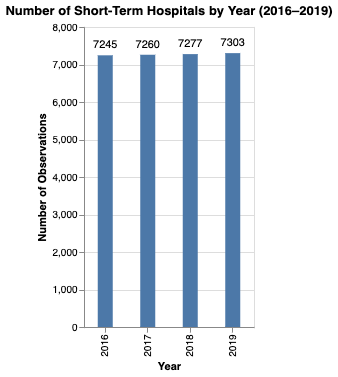
\includegraphics{1-3.png}

}

\caption{Number of short term hospitals by year}

\end{figure}%

\begin{enumerate}
\def\labelenumi{\arabic{enumi}.}
\setcounter{enumi}{3}
\tightlist
\item
\end{enumerate}

\begin{enumerate}
\def\labelenumi{\alph{enumi}.}
\tightlist
\item
\end{enumerate}

\begin{Shaded}
\begin{Highlighting}[]
\NormalTok{unique\_hospitals\_by\_year }\OperatorTok{=}\NormalTok{ pos\_all.groupby(}\StringTok{\textquotesingle{}Year\textquotesingle{}}\NormalTok{)[}\StringTok{\textquotesingle{}PRVDR\_NUM\textquotesingle{}}\NormalTok{].nunique().reset\_index(name}\OperatorTok{=}\StringTok{\textquotesingle{}Unique\_Hospitals\textquotesingle{}}\NormalTok{)}


\NormalTok{unique\_hospitals\_chart }\OperatorTok{=}\NormalTok{ alt.Chart(unique\_hospitals\_by\_year).mark\_bar(size}\OperatorTok{=}\DecValTok{30}\NormalTok{).encode(x}\OperatorTok{=}\NormalTok{alt.X(}\StringTok{\textquotesingle{}Year:O\textquotesingle{}}\NormalTok{, title}\OperatorTok{=}\StringTok{\textquotesingle{}Year\textquotesingle{}}\NormalTok{),  }
\NormalTok{y}\OperatorTok{=}\NormalTok{alt.Y(}\StringTok{\textquotesingle{}Unique\_Hospitals:Q\textquotesingle{}}\NormalTok{, title}\OperatorTok{=}\StringTok{\textquotesingle{}Number of Unique Hospitals\textquotesingle{}}\NormalTok{),}
\NormalTok{    tooltip}\OperatorTok{=}\NormalTok{[}\StringTok{\textquotesingle{}Year\textquotesingle{}}\NormalTok{, }\StringTok{\textquotesingle{}Unique\_Hospitals\textquotesingle{}}\NormalTok{] ).properties(}
\NormalTok{        width }\OperatorTok{=} \DecValTok{170}\NormalTok{,}
\NormalTok{         title}\OperatorTok{=}\StringTok{"Number of Unique Short{-}Term Hospitals by Year (2016–2019)"}\NormalTok{)}

\NormalTok{unique\_hospitals\_chart}
\end{Highlighting}
\end{Shaded}

\begin{verbatim}
alt.Chart(...)
\end{verbatim}

\begin{figure}[H]

{\centering 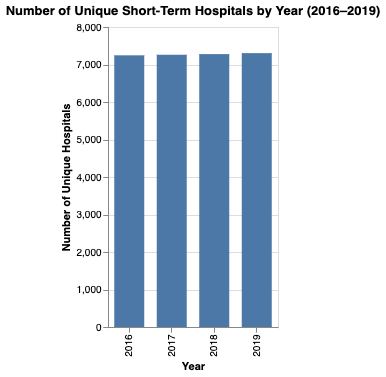
\includegraphics{1-4.png}

}

\caption{Number of Unique Short-term hospitals by year}

\end{figure}%

\begin{enumerate}
\def\labelenumi{\alph{enumi}.}
\setcounter{enumi}{1}
\tightlist
\item
\end{enumerate}

The presence of multiple entries for some hospitals in the same year
suggests that hospitals may have multiple records within a year. This
could be due to:

Multiple service types or specializations under the same certification
number.

Data entries from different quarters if the dataset was compiled from
quarterly reports.

Administrative updates that result in duplicate entries for the same
hospital.

\subsection{Identify hospital closures in POS file (15 pts)
(*)}\label{identify-hospital-closures-in-pos-file-15-pts}

\begin{enumerate}
\def\labelenumi{\arabic{enumi}.}
\tightlist
\item
\end{enumerate}

\section{Finding closures based on
`PRVDR\_NUM'}\label{finding-closures-based-on-prvdr_num}

\begin{Shaded}
\begin{Highlighting}[]
\ImportTok{import}\NormalTok{ pandas }\ImportTok{as}\NormalTok{ pd}

\NormalTok{pos2016 }\OperatorTok{=}\NormalTok{ pd.read\_csv(}\StringTok{"POS\_File\_Hospital\_Non\_Hospital\_Facilities\_Q4\_2016.csv"}\NormalTok{, encoding}\OperatorTok{=}\StringTok{"ISO{-}8859{-}1"}\NormalTok{)}
\NormalTok{pos2017 }\OperatorTok{=}\NormalTok{ pd.read\_csv(}\StringTok{"POS\_File\_Hospital\_Non\_Hospital\_Facilities\_Q4\_2017.csv"}\NormalTok{, encoding}\OperatorTok{=}\StringTok{"ISO{-}8859{-}1"}\NormalTok{)}
\NormalTok{pos2018 }\OperatorTok{=}\NormalTok{ pd.read\_csv(}\StringTok{"POS\_File\_Hospital\_Non\_Hospital\_Facilities\_Q4\_2018.csv"}\NormalTok{, encoding}\OperatorTok{=}\StringTok{"ISO{-}8859{-}1"}\NormalTok{)}
\NormalTok{pos2019 }\OperatorTok{=}\NormalTok{ pd.read\_csv(}\StringTok{"POS\_File\_Hospital\_Non\_Hospital\_Facilities\_Q4\_2019.csv"}\NormalTok{, encoding}\OperatorTok{=}\StringTok{"ISO{-}8859{-}1"}\NormalTok{)}

\BuiltInTok{print}\NormalTok{(}\StringTok{"Columns in 2016 data:"}\NormalTok{, pos2016.columns.tolist())}

\NormalTok{active\_2016 }\OperatorTok{=}\NormalTok{ pos2016[[}\StringTok{\textquotesingle{}FAC\_NAME\textquotesingle{}}\NormalTok{, }\StringTok{\textquotesingle{}ZIP\_CD\textquotesingle{}}\NormalTok{,}\StringTok{\textquotesingle{}STATE\_CD\textquotesingle{}}\NormalTok{,}\StringTok{\textquotesingle{}PRVDR\_NUM\textquotesingle{}}\NormalTok{]].copy()}

\KeywordTok{def}\NormalTok{ find\_closures(active\_df, }\OperatorTok{*}\NormalTok{args):}
\NormalTok{    closures }\OperatorTok{=}\NormalTok{ active\_df.copy()}
\NormalTok{    closures[}\StringTok{\textquotesingle{}Suspected\_Closure\_Year\textquotesingle{}}\NormalTok{] }\OperatorTok{=} \VariableTok{None}

    \ControlFlowTok{for}\NormalTok{ year, df }\KeywordTok{in} \BuiltInTok{enumerate}\NormalTok{(args, start}\OperatorTok{=}\DecValTok{2017}\NormalTok{):}
\NormalTok{        closures.loc[}\OperatorTok{\textasciitilde{}}\NormalTok{closures[}\StringTok{\textquotesingle{}PRVDR\_NUM\textquotesingle{}}\NormalTok{].isin(df[}\StringTok{\textquotesingle{}PRVDR\_NUM\textquotesingle{}}\NormalTok{]), }\StringTok{\textquotesingle{}Suspected\_Closure\_Year\textquotesingle{}}\NormalTok{] }\OperatorTok{=}\NormalTok{ year}

    \ControlFlowTok{return}\NormalTok{ closures.dropna(subset}\OperatorTok{=}\NormalTok{[}\StringTok{\textquotesingle{}Suspected\_Closure\_Year\textquotesingle{}}\NormalTok{])}

\NormalTok{suspected\_closures }\OperatorTok{=}\NormalTok{ find\_closures(active\_2016, pos2017, pos2018, pos2019)}

\BuiltInTok{print}\NormalTok{(}\StringTok{"Total suspected closures:"}\NormalTok{, }\BuiltInTok{len}\NormalTok{(suspected\_closures))}
\BuiltInTok{print}\NormalTok{(suspected\_closures.sort\_values(}\StringTok{\textquotesingle{}FAC\_NAME\textquotesingle{}}\NormalTok{).head(}\DecValTok{10}\NormalTok{))}
\end{Highlighting}
\end{Shaded}

\begin{verbatim}
Columns in 2016 data: ['PRVDR_CTGRY_SBTYP_CD', 'PRVDR_CTGRY_CD', 'CITY_NAME', 'FAC_NAME', 'PRVDR_NUM', 'STATE_CD', 'ZIP_CD']
Total suspected closures: 3
                                                 FAC_NAME   ZIP_CD STATE_CD  \
11268   ADVENTIST HEALTH COMMUNITY CARE-REEDLEY WOMEN'...  93654.0       CA   
117766                        REHABILITATION & HEALTHCARE  77521.0       TX   
68832                    VETERANS ADMINISTRATION HOSPITAL  63125.0       MO   

       PRVDR_NUM Suspected_Closure_Year  
11268     058985                   2019  
117766    45F481                   2019  
68832     262307                   2019  
\end{verbatim}

There are 3 hospitals that fit this definition.

\begin{enumerate}
\def\labelenumi{\arabic{enumi}.}
\setcounter{enumi}{1}
\tightlist
\item
\end{enumerate}

\begin{Shaded}
\begin{Highlighting}[]
\BuiltInTok{print}\NormalTok{(suspected\_closures.sort\_values(}\StringTok{\textquotesingle{}FAC\_NAME\textquotesingle{}}\NormalTok{)[[}\StringTok{\textquotesingle{}FAC\_NAME\textquotesingle{}}\NormalTok{, }\StringTok{\textquotesingle{}Suspected\_Closure\_Year\textquotesingle{}}\NormalTok{]].head(}\DecValTok{10}\NormalTok{))}
\end{Highlighting}
\end{Shaded}

\begin{verbatim}
                                                 FAC_NAME  \
11268   ADVENTIST HEALTH COMMUNITY CARE-REEDLEY WOMEN'...   
117766                        REHABILITATION & HEALTHCARE   
68832                    VETERANS ADMINISTRATION HOSPITAL   

       Suspected_Closure_Year  
11268                    2019  
117766                   2019  
68832                    2019  
\end{verbatim}

\begin{enumerate}
\def\labelenumi{\arabic{enumi}.}
\setcounter{enumi}{2}
\tightlist
\item
\end{enumerate}

\begin{Shaded}
\begin{Highlighting}[]
\NormalTok{zip\_counts\_2016 }\OperatorTok{=}\NormalTok{ pos2016.groupby(}\StringTok{\textquotesingle{}ZIP\_CD\textquotesingle{}}\NormalTok{).size()}
\NormalTok{zip\_counts\_2017 }\OperatorTok{=}\NormalTok{ pos2017.groupby(}\StringTok{\textquotesingle{}ZIP\_CD\textquotesingle{}}\NormalTok{).size()}
\NormalTok{zip\_counts\_2018 }\OperatorTok{=}\NormalTok{ pos2018.groupby(}\StringTok{\textquotesingle{}ZIP\_CD\textquotesingle{}}\NormalTok{).size()}
\NormalTok{zip\_counts\_2019 }\OperatorTok{=}\NormalTok{ pos2019.groupby(}\StringTok{\textquotesingle{}ZIP\_CD\textquotesingle{}}\NormalTok{).size()}

\NormalTok{suspected\_closures[}\StringTok{\textquotesingle{}is\_merger\textquotesingle{}}\NormalTok{] }\OperatorTok{=}\NormalTok{ suspected\_closures.}\BuiltInTok{apply}\NormalTok{(}
    \KeywordTok{lambda}\NormalTok{ row: (}
\NormalTok{        zip\_counts\_2016.get(row[}\StringTok{\textquotesingle{}ZIP\_CD\textquotesingle{}}\NormalTok{], }\DecValTok{0}\NormalTok{) }\OperatorTok{==}\NormalTok{ zip\_counts\_2017.get(row[}\StringTok{\textquotesingle{}ZIP\_CD\textquotesingle{}}\NormalTok{], }\DecValTok{0}\NormalTok{) }\KeywordTok{or}
\NormalTok{        zip\_counts\_2017.get(row[}\StringTok{\textquotesingle{}ZIP\_CD\textquotesingle{}}\NormalTok{], }\DecValTok{0}\NormalTok{) }\OperatorTok{==}\NormalTok{ zip\_counts\_2018.get(row[}\StringTok{\textquotesingle{}ZIP\_CD\textquotesingle{}}\NormalTok{], }\DecValTok{0}\NormalTok{) }\KeywordTok{or}
\NormalTok{        zip\_counts\_2018.get(row[}\StringTok{\textquotesingle{}ZIP\_CD\textquotesingle{}}\NormalTok{], }\DecValTok{0}\NormalTok{) }\OperatorTok{==}\NormalTok{ zip\_counts\_2019.get(row[}\StringTok{\textquotesingle{}ZIP\_CD\textquotesingle{}}\NormalTok{], }\DecValTok{0}\NormalTok{)}
\NormalTok{    ), axis}\OperatorTok{=}\DecValTok{1}
\NormalTok{)}

\NormalTok{filtered\_closures }\OperatorTok{=}\NormalTok{ suspected\_closures[}\OperatorTok{\textasciitilde{}}\NormalTok{suspected\_closures[}\StringTok{\textquotesingle{}is\_merger\textquotesingle{}}\NormalTok{]]}

\BuiltInTok{print}\NormalTok{(}\StringTok{"Total closures after filtering mergers:"}\NormalTok{, }\BuiltInTok{len}\NormalTok{(filtered\_closures))}
\BuiltInTok{print}\NormalTok{(filtered\_closures.sort\_values(}\StringTok{\textquotesingle{}FAC\_NAME\textquotesingle{}}\NormalTok{)[[}\StringTok{\textquotesingle{}FAC\_NAME\textquotesingle{}}\NormalTok{, }\StringTok{\textquotesingle{}ZIP\_CD\textquotesingle{}}\NormalTok{, }\StringTok{\textquotesingle{}Suspected\_Closure\_Year\textquotesingle{}}\NormalTok{]].head(}\DecValTok{10}\NormalTok{))}
\end{Highlighting}
\end{Shaded}

\begin{verbatim}
Total closures after filtering mergers: 0
Empty DataFrame
Columns: [FAC_NAME, ZIP_CD, Suspected_Closure_Year]
Index: []
\end{verbatim}

\begin{verbatim}
a. Among the suspected closures, how many hospitals fit this definition of potentially being a merger/acquisition?
b. After filtering out these potential mergers or acquisitions, 0 hospitals remain in the list of closures.
c. Since there are no remaining hospitals after filtering, the sorted list of corrected hospital closures is empty.
\end{verbatim}

\subsection{Download Census zip code shapefile (10
pt)}\label{download-census-zip-code-shapefile-10-pt}

\begin{enumerate}
\def\labelenumi{\arabic{enumi}.}
\item
  \begin{enumerate}
  \def\labelenumii{\alph{enumii}.}
  \tightlist
  \item
  \end{enumerate}

  The five type of files are shp, dbf, shx, prj and xml. .shp
  (Shapefile) - The main file containing the geometry of shapes, such as
  points, lines, or polygons, for geographic features like ZIP code
  boundaries.

  .shx (Shape Index Format) - An index file that enables quick access to
  the geometry data in the .shp file.

  .dbf (dBASE Table) - A table file containing attribute data for each
  shape, including properties like ZIP codes, which complements the .shp
  file for map creation.

  .prj (Projection) - A file that defines the projection and coordinate
  system, ensuring geographic data aligns correctly with other spatial
  datasets.

  .xml (Metadata) - A metadata file that provides information about the
  dataset, including its source, creation date, and content details.

  \begin{enumerate}
  \def\labelenumii{\alph{enumii}.}
  \setcounter{enumii}{1}
  \tightlist
  \item
  \end{enumerate}

  The largest file is the .shp file (837.5 MB), as it contains the
  geometry data. The .dbf file (6.4 MB) is the next largest, containing
  attribute information. The .shx file (265 KB) is smaller, as it only
  contains an index. The .prj file (165 bytes) and the .xml file (16 KB)
  are small because they only contain projection and metadata
  information.
\item
\end{enumerate}

\begin{Shaded}
\begin{Highlighting}[]
\ImportTok{import}\NormalTok{ geopandas }\ImportTok{as}\NormalTok{ gpd}

\NormalTok{zip\_codes }\OperatorTok{=}\NormalTok{ gpd.read\_file(}\StringTok{"gz\_2010\_us\_860\_00\_500k.shp"}\NormalTok{, engine }\OperatorTok{=} \StringTok{"pyogrio"}\NormalTok{)}

\CommentTok{\# Display the first few rows to confirm loading}
\BuiltInTok{print}\NormalTok{(zip\_codes.head())}
\end{Highlighting}
\end{Shaded}

\begin{verbatim}
           GEO_ID  ZCTA5   NAME   LSAD  CENSUSAREA  \
0  8600000US01040  01040  01040  ZCTA5      21.281   
1  8600000US01050  01050  01050  ZCTA5      38.329   
2  8600000US01053  01053  01053  ZCTA5       5.131   
3  8600000US01056  01056  01056  ZCTA5      27.205   
4  8600000US01057  01057  01057  ZCTA5      44.907   

                                            geometry  
0  POLYGON ((-72.62734 42.16203, -72.62764 42.162...  
1  POLYGON ((-72.95393 42.34379, -72.95385 42.343...  
2  POLYGON ((-72.68286 42.37002, -72.68287 42.369...  
3  POLYGON ((-72.39529 42.18476, -72.39653 42.183...  
4  MULTIPOLYGON (((-72.39191 42.08066, -72.39077 ...  
\end{verbatim}

\begin{Shaded}
\begin{Highlighting}[]
\ImportTok{import}\NormalTok{ json}
\end{Highlighting}
\end{Shaded}

\begin{Shaded}
\begin{Highlighting}[]
\NormalTok{texas\_zip\_codes }\OperatorTok{=}\NormalTok{ zip\_codes[zip\_codes[}\StringTok{\textquotesingle{}ZCTA5\textquotesingle{}}\NormalTok{].}\BuiltInTok{str}\NormalTok{.startswith((}\StringTok{\textquotesingle{}75\textquotesingle{}}\NormalTok{, }\StringTok{\textquotesingle{}76\textquotesingle{}}\NormalTok{, }\StringTok{\textquotesingle{}77\textquotesingle{}}\NormalTok{, }\StringTok{\textquotesingle{}78\textquotesingle{}}\NormalTok{))]}

\NormalTok{pos2016[}\StringTok{\textquotesingle{}ZIP\_CD\textquotesingle{}}\NormalTok{] }\OperatorTok{=}\NormalTok{ pos2016[}\StringTok{\textquotesingle{}ZIP\_CD\textquotesingle{}}\NormalTok{].astype(}\BuiltInTok{str}\NormalTok{).}\BuiltInTok{str}\NormalTok{.replace(}\StringTok{\textquotesingle{}.0\textquotesingle{}}\NormalTok{, }\StringTok{\textquotesingle{}\textquotesingle{}}\NormalTok{, regex}\OperatorTok{=}\VariableTok{False}\NormalTok{)}

\NormalTok{hospitals\_count }\OperatorTok{=}\NormalTok{ pos2016[}\StringTok{\textquotesingle{}ZIP\_CD\textquotesingle{}}\NormalTok{].value\_counts().reset\_index()}
\NormalTok{hospitals\_count.columns }\OperatorTok{=}\NormalTok{ [}\StringTok{\textquotesingle{}ZCTA5\textquotesingle{}}\NormalTok{, }\StringTok{\textquotesingle{}hospital\_count\textquotesingle{}}\NormalTok{]}

\NormalTok{texas\_hospitals }\OperatorTok{=}\NormalTok{ texas\_zip\_codes.merge(hospitals\_count, on}\OperatorTok{=}\StringTok{\textquotesingle{}ZCTA5\textquotesingle{}}\NormalTok{, how}\OperatorTok{=}\StringTok{\textquotesingle{}left\textquotesingle{}}\NormalTok{).fillna(}\DecValTok{0}\NormalTok{)}
\NormalTok{texas\_hospitals[}\StringTok{\textquotesingle{}hospital\_count\textquotesingle{}}\NormalTok{] }\OperatorTok{=}\NormalTok{ texas\_hospitals[}\StringTok{\textquotesingle{}hospital\_count\textquotesingle{}}\NormalTok{].astype(}\BuiltInTok{int}\NormalTok{)}

\BuiltInTok{print}\NormalTok{(texas\_hospitals[[}\StringTok{\textquotesingle{}ZCTA5\textquotesingle{}}\NormalTok{, }\StringTok{\textquotesingle{}hospital\_count\textquotesingle{}}\NormalTok{]].head()) }

\NormalTok{texas\_hospitals }\OperatorTok{=}\NormalTok{ texas\_hospitals.to\_crs(}\StringTok{"EPSG:4326"}\NormalTok{)}
\NormalTok{geojson\_data }\OperatorTok{=}\NormalTok{ json.loads(texas\_hospitals.to\_json())}

\NormalTok{choropleth }\OperatorTok{=}\NormalTok{ alt.Chart(alt.Data(values}\OperatorTok{=}\NormalTok{geojson\_data[}\StringTok{\textquotesingle{}features\textquotesingle{}}\NormalTok{])).mark\_geoshape().encode(}
\NormalTok{    color}\OperatorTok{=}\NormalTok{alt.Color(}\StringTok{\textquotesingle{}properties.hospital\_count:Q\textquotesingle{}}\NormalTok{, title}\OperatorTok{=}\StringTok{"Number of Hospitals"}\NormalTok{),}
\NormalTok{    tooltip}\OperatorTok{=}\NormalTok{[}
\NormalTok{        alt.Tooltip(}\StringTok{\textquotesingle{}properties.ZCTA5:O\textquotesingle{}}\NormalTok{, title}\OperatorTok{=}\StringTok{"ZIP Code"}\NormalTok{),}
\NormalTok{        alt.Tooltip(}\StringTok{\textquotesingle{}properties.hospital\_count:Q\textquotesingle{}}\NormalTok{, title}\OperatorTok{=}\StringTok{"Hospital Count"}\NormalTok{)}
        
\NormalTok{    ]}
\NormalTok{).properties(}
\NormalTok{    width}\OperatorTok{=}\DecValTok{300}\NormalTok{,}
\NormalTok{    height}\OperatorTok{=}\DecValTok{400}\NormalTok{,}
\NormalTok{    title}\OperatorTok{=}\StringTok{"Hospitals per ZIP Code in Texas (2016)"}
\NormalTok{)}

\NormalTok{choropleth}
\end{Highlighting}
\end{Shaded}

\begin{verbatim}
   ZCTA5  hospital_count
0  78624              21
1  78626              25
2  78628              11
3  78631               0
4  78632               0
\end{verbatim}

\begin{verbatim}
alt.Chart(...)
\end{verbatim}

\begin{figure}[H]

{\centering 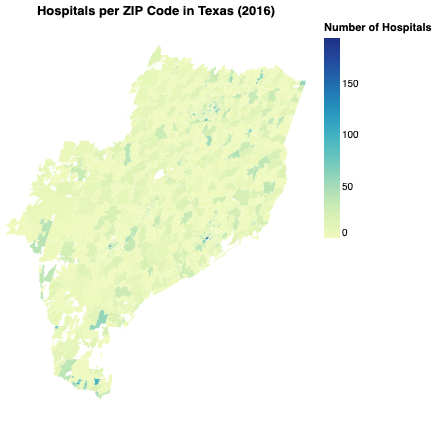
\includegraphics{3-2.png}

}

\caption{Choropleth}

\end{figure}%

\subsection{Calculate zip code's distance to the nearest hospital (20
pts)
(*)}\label{calculate-zip-codes-distance-to-the-nearest-hospital-20-pts}

\begin{enumerate}
\def\labelenumi{\arabic{enumi}.}
\tightlist
\item
\end{enumerate}

\begin{Shaded}
\begin{Highlighting}[]
\NormalTok{zip\_codes[}\StringTok{\textquotesingle{}centroid\textquotesingle{}}\NormalTok{] }\OperatorTok{=}\NormalTok{ zip\_codes.geometry.centroid}
\NormalTok{zips\_all\_centroids }\OperatorTok{=}\NormalTok{ zip\_codes[[}\StringTok{\textquotesingle{}ZCTA5\textquotesingle{}}\NormalTok{, }\StringTok{\textquotesingle{}centroid\textquotesingle{}}\NormalTok{]]}
\BuiltInTok{print}\NormalTok{(}\SpecialStringTok{f"Dimensions of zips\_all\_centroids: }\SpecialCharTok{\{}\NormalTok{zips\_all\_centroids}\SpecialCharTok{.}\NormalTok{shape}\SpecialCharTok{\}}\SpecialStringTok{"}\NormalTok{)}
\end{Highlighting}
\end{Shaded}

\begin{verbatim}
/var/folders/gc/ws7810v915ng_kb_x8xx72n80000gn/T/ipykernel_84505/2749478377.py:1: UserWarning: Geometry is in a geographic CRS. Results from 'centroid' are likely incorrect. Use 'GeoSeries.to_crs()' to re-project geometries to a projected CRS before this operation.

  zip_codes['centroid'] = zip_codes.geometry.centroid
\end{verbatim}

\begin{verbatim}
Dimensions of zips_all_centroids: (33120, 2)
\end{verbatim}

\begin{enumerate}
\def\labelenumi{\arabic{enumi}.}
\setcounter{enumi}{1}
\tightlist
\item
\end{enumerate}

\begin{Shaded}
\begin{Highlighting}[]
\NormalTok{texas\_prefixes }\OperatorTok{=}\NormalTok{ (}\StringTok{\textquotesingle{}75\textquotesingle{}}\NormalTok{, }\StringTok{\textquotesingle{}76\textquotesingle{}}\NormalTok{, }\StringTok{\textquotesingle{}77\textquotesingle{}}\NormalTok{, }\StringTok{\textquotesingle{}78\textquotesingle{}}\NormalTok{)}
\NormalTok{border\_states\_prefixes }\OperatorTok{=}\NormalTok{ texas\_prefixes }\OperatorTok{+}\NormalTok{ (}\StringTok{\textquotesingle{}70\textquotesingle{}}\NormalTok{, }\StringTok{\textquotesingle{}71\textquotesingle{}}\NormalTok{, }\StringTok{\textquotesingle{}72\textquotesingle{}}\NormalTok{, }\StringTok{\textquotesingle{}73\textquotesingle{}}\NormalTok{, }\StringTok{\textquotesingle{}79\textquotesingle{}}\NormalTok{, }\StringTok{\textquotesingle{}80\textquotesingle{}}\NormalTok{, }\StringTok{\textquotesingle{}81\textquotesingle{}}\NormalTok{, }\StringTok{\textquotesingle{}82\textquotesingle{}}\NormalTok{)}

\NormalTok{zips\_texas\_centroids }\OperatorTok{=}\NormalTok{ zips\_all\_centroids[zips\_all\_centroids[}\StringTok{\textquotesingle{}ZCTA5\textquotesingle{}}\NormalTok{].}\BuiltInTok{str}\NormalTok{.startswith(texas\_prefixes)]}
\NormalTok{zips\_texas\_borderstates\_centroids }\OperatorTok{=}\NormalTok{ zips\_all\_centroids[zips\_all\_centroids[}\StringTok{\textquotesingle{}ZCTA5\textquotesingle{}}\NormalTok{].}\BuiltInTok{str}\NormalTok{.startswith(border\_states\_prefixes)]}

\BuiltInTok{print}\NormalTok{(}\SpecialStringTok{f"Unique ZIP codes in Texas subset: }\SpecialCharTok{\{}\NormalTok{zips\_texas\_centroids[}\StringTok{\textquotesingle{}ZCTA5\textquotesingle{}}\NormalTok{]}\SpecialCharTok{.}\NormalTok{nunique()}\SpecialCharTok{\}}\SpecialStringTok{"}\NormalTok{)}
\BuiltInTok{print}\NormalTok{(}\SpecialStringTok{f"Unique ZIP codes in Texas and bordering states subset: }\SpecialCharTok{\{}\NormalTok{zips\_texas\_borderstates\_centroids[}\StringTok{\textquotesingle{}ZCTA5\textquotesingle{}}\NormalTok{]}\SpecialCharTok{.}\NormalTok{nunique()}\SpecialCharTok{\}}\SpecialStringTok{"}\NormalTok{)}
\end{Highlighting}
\end{Shaded}

\begin{verbatim}
Unique ZIP codes in Texas subset: 1614
Unique ZIP codes in Texas and bordering states subset: 4034
\end{verbatim}

\begin{enumerate}
\def\labelenumi{\arabic{enumi}.}
\setcounter{enumi}{2}
\tightlist
\item
\end{enumerate}

\begin{Shaded}
\begin{Highlighting}[]
\NormalTok{pos2016[}\StringTok{\textquotesingle{}ZIP\_CD\textquotesingle{}}\NormalTok{] }\OperatorTok{=}\NormalTok{ pos2016[}\StringTok{\textquotesingle{}ZIP\_CD\textquotesingle{}}\NormalTok{].astype(}\BuiltInTok{str}\NormalTok{).}\BuiltInTok{str}\NormalTok{.zfill(}\DecValTok{5}\NormalTok{)}
\NormalTok{hospitals\_in\_2016 }\OperatorTok{=}\NormalTok{ pos2016[[}\StringTok{\textquotesingle{}ZIP\_CD\textquotesingle{}}\NormalTok{]].drop\_duplicates()}

\NormalTok{zips\_withhospital\_centroids }\OperatorTok{=}\NormalTok{ zips\_texas\_borderstates\_centroids.merge(}
\NormalTok{    hospitals\_in\_2016, left\_on}\OperatorTok{=}\StringTok{\textquotesingle{}ZCTA5\textquotesingle{}}\NormalTok{, right\_on}\OperatorTok{=}\StringTok{\textquotesingle{}ZIP\_CD\textquotesingle{}}\NormalTok{, how}\OperatorTok{=}\StringTok{\textquotesingle{}inner\textquotesingle{}}
\NormalTok{)}
\BuiltInTok{print}\NormalTok{(}\SpecialStringTok{f"Total ZIP codes with at least one hospital: }\SpecialCharTok{\{}\BuiltInTok{len}\NormalTok{(zips\_withhospital\_centroids)}\SpecialCharTok{\}}\SpecialStringTok{"}\NormalTok{)}
\end{Highlighting}
\end{Shaded}

\begin{verbatim}
Total ZIP codes with at least one hospital: 2216
\end{verbatim}

\begin{enumerate}
\def\labelenumi{\arabic{enumi}.}
\setcounter{enumi}{3}
\tightlist
\item
\end{enumerate}

\begin{enumerate}
\def\labelenumi{\alph{enumi}.}
\tightlist
\item
\end{enumerate}

\begin{Shaded}
\begin{Highlighting}[]
\ImportTok{import}\NormalTok{ time}
\ImportTok{from}\NormalTok{ shapely.geometry }\ImportTok{import}\NormalTok{ Point}
\ImportTok{from}\NormalTok{ geopy.distance }\ImportTok{import}\NormalTok{ geodesic}
\CommentTok{\# 1.4a Calculate distance for a subset of 10 zip codes}
\NormalTok{subset\_zips }\OperatorTok{=}\NormalTok{ zips\_texas\_centroids.head(}\DecValTok{10}\NormalTok{)}
\NormalTok{start\_time }\OperatorTok{=}\NormalTok{ time.time()}

\NormalTok{subset\_zips[}\StringTok{\textquotesingle{}nearest\_hospital\_dist\textquotesingle{}}\NormalTok{] }\OperatorTok{=}\NormalTok{ subset\_zips[}\StringTok{\textquotesingle{}centroid\textquotesingle{}}\NormalTok{].}\BuiltInTok{apply}\NormalTok{(}
    \KeywordTok{lambda}\NormalTok{ zip\_point: zips\_withhospital\_centroids[}\StringTok{\textquotesingle{}centroid\textquotesingle{}}\NormalTok{].}\BuiltInTok{apply}\NormalTok{(}
        \KeywordTok{lambda}\NormalTok{ hospital\_point: geodesic(}
\NormalTok{            (zip\_point.y, zip\_point.x), }
\NormalTok{            (hospital\_point.y, hospital\_point.x)}
\NormalTok{        ).miles}
\NormalTok{    ).}\BuiltInTok{min}\NormalTok{()}
\NormalTok{)}

\NormalTok{subset\_time }\OperatorTok{=}\NormalTok{ time.time() }\OperatorTok{{-}}\NormalTok{ start\_time}
\BuiltInTok{print}\NormalTok{(}\SpecialStringTok{f"Time taken for subset (10 ZIP codes): }\SpecialCharTok{\{}\NormalTok{subset\_time}\SpecialCharTok{\}}\SpecialStringTok{ seconds"}\NormalTok{)}
\end{Highlighting}
\end{Shaded}

\begin{verbatim}
Time taken for subset (10 ZIP codes): 2.8513271808624268 seconds
\end{verbatim}

\begin{verbatim}
/Users/mengyuting/Documents/GitHub/problem-set-4-yuting-yunzhou/.venv/lib/python3.8/site-packages/geopandas/geodataframe.py:1538: SettingWithCopyWarning: 
A value is trying to be set on a copy of a slice from a DataFrame.
Try using .loc[row_indexer,col_indexer] = value instead

See the caveats in the documentation: https://pandas.pydata.org/pandas-docs/stable/user_guide/indexing.html#returning-a-view-versus-a-copy
  super().__setitem__(key, value)
\end{verbatim}

It is faster than what I expected, around 5 seconds.

\begin{enumerate}
\def\labelenumi{\alph{enumi}.}
\setcounter{enumi}{1}
\tightlist
\item
\end{enumerate}

start\_time = time.time()

zips\_texas\_centroids{[}`nearest\_hospital\_dist'{]} =
zips\_texas\_centroids{[}`centroid'{]}.apply( lambda zip\_point:
zips\_withhospital\_centroids{[}`centroid'{]}.apply( lambda
hospital\_point: geodesic( (zip\_point.y, zip\_point.x),
(hospital\_point.y, hospital\_point.x) ).miles ).min() )

full\_time = time.time() - start\_time print(f''Total time for full
calculation: \{full\_time\} seconds'')

\begin{enumerate}
\def\labelenumi{\alph{enumi}.}
\setcounter{enumi}{2}
\tightlist
\item
\end{enumerate}

\begin{Shaded}
\begin{Highlighting}[]
\BuiltInTok{print}\NormalTok{(zip\_codes.crs)}
\end{Highlighting}
\end{Shaded}

\begin{verbatim}
EPSG:4269
\end{verbatim}

The units are in latitude and longitude in degrees as units.

\begin{Shaded}
\begin{Highlighting}[]
\BuiltInTok{print}\NormalTok{(}\StringTok{"Columns in zips\_texas\_centroids:"}\NormalTok{, zips\_texas\_centroids.columns)}
\BuiltInTok{print}\NormalTok{(zips\_texas\_centroids.head())}

\BuiltInTok{print}\NormalTok{(}\StringTok{"Columns in zips\_withhospital\_centroids:"}\NormalTok{, zips\_withhospital\_centroids.columns)}
\BuiltInTok{print}\NormalTok{(zips\_withhospital\_centroids.head())}
\end{Highlighting}
\end{Shaded}

\begin{verbatim}
Columns in zips_texas_centroids: Index(['ZCTA5', 'centroid'], dtype='object')
      ZCTA5                    centroid
9207  78624  POINT (-98.87707 30.28160)
9208  78626  POINT (-97.59733 30.66535)
9209  78628  POINT (-97.75112 30.64108)
9210  78631  POINT (-99.30528 30.33772)
9211  78632  POINT (-97.47045 29.69633)
Columns in zips_withhospital_centroids: Index(['ZCTA5', 'centroid', 'ZIP_CD'], dtype='object')
   ZCTA5                    centroid ZIP_CD
0  70003  POINT (-90.21397 29.99864)  70003
1  70032  POINT (-89.99779 29.95816)  70032
2  70039  POINT (-90.38906 29.88151)  70039
3  70043  POINT (-89.96276 29.94804)  70043
4  70047  POINT (-90.36588 29.96953)  70047
\end{verbatim}

zips\_texas\_centroids = gpd.GeoDataFrame(zips\_texas\_centroids,
geometry=`centroid') zips\_withhospital\_centroids =
gpd.GeoDataFrame(zips\_withhospital\_centroids, geometry=`centroid')

zips\_texas\_centroids = zips\_texas\_centroids.to\_crs(``EPSG:3857'')
zips\_withhospital\_centroids =
zips\_withhospital\_centroids.to\_crs(``EPSG:3857'')

def calculate\_nearest\_distance(row, hospitals\_gdf): nearest\_geom =
nearest\_points(row.geometry, hospitals\_gdf.unary\_union){[}1{]}
distance\_meters = row.geometry.distance(nearest\_geom) distance\_miles
= distance\_meters * 0.000621371\\
return distance\_miles

zips\_texas\_centroids{[}`nearest\_hospital\_dist\_miles'{]} =
zips\_texas\_centroids.apply( calculate\_nearest\_distance,
hospitals\_gdf=zips\_withhospital\_centroids, axis=1 )

from shapely.ops import nearest\_points def
calculate\_nearest\_distance(row, hospitals\_gdf): \# Find the nearest
point in hospitals\_gdf for each ZIP code point nearest\_geom =
nearest\_points(row.geometry, hospitals\_gdf.unary\_union){[}1{]} \#
Calculate the distance in meters and convert to miles distance\_meters =
row.geometry.distance(nearest\_geom) distance\_miles = distance\_meters
* 0.000621371 \# Convert meters to miles return distance\_miles

zips\_texas\_centroids{[}`nearest\_hospital\_dist\_miles'{]} =
zips\_texas\_centroids.apply( calculate\_nearest\_distance,
hospitals\_gdf=zips\_withhospital\_centroids, axis=1 )

print(zips\_texas\_centroids{[}{[}`ZCTA5',
`nearest\_hospital\_dist\_miles'{]}{]})

I am not able to run this code chunk since it keeps giving me error
message of ``geometry.''

\subsection{Effects of closures on access in Texas (15
pts)}\label{effects-of-closures-on-access-in-texas-15-pts}

\begin{enumerate}
\def\labelenumi{\arabic{enumi}.}
\tightlist
\item
\end{enumerate}

\begin{Shaded}
\begin{Highlighting}[]
\ControlFlowTok{for}\NormalTok{ year, pos\_data }\KeywordTok{in} \BuiltInTok{zip}\NormalTok{([}\DecValTok{2017}\NormalTok{, }\DecValTok{2018}\NormalTok{, }\DecValTok{2019}\NormalTok{], [pos2017, pos2018, pos2019]):}
\NormalTok{    duplicates }\OperatorTok{=}\NormalTok{ pos\_data[}\StringTok{\textquotesingle{}PRVDR\_NUM\textquotesingle{}}\NormalTok{].duplicated().}\BuiltInTok{sum}\NormalTok{()}
    \BuiltInTok{print}\NormalTok{(}\SpecialStringTok{f"Year }\SpecialCharTok{\{}\NormalTok{year}\SpecialCharTok{\}}\SpecialStringTok{: }\SpecialCharTok{\{}\NormalTok{duplicates}\SpecialCharTok{\}}\SpecialStringTok{ duplicates found in PRVDR\_NUM"}\NormalTok{)}

\KeywordTok{def}\NormalTok{ find\_closures\_with\_merger\_check(active\_df, }\OperatorTok{*}\NormalTok{args):}
\NormalTok{    closures }\OperatorTok{=}\NormalTok{ active\_df.copy()}
\NormalTok{    closures[}\StringTok{\textquotesingle{}Suspected\_Closure\_Year\textquotesingle{}}\NormalTok{] }\OperatorTok{=} \VariableTok{None}

    \ControlFlowTok{for}\NormalTok{ year, df }\KeywordTok{in} \BuiltInTok{enumerate}\NormalTok{(args, start}\OperatorTok{=}\DecValTok{2017}\NormalTok{):}
\NormalTok{        df\_unique }\OperatorTok{=}\NormalTok{ df.drop\_duplicates(subset}\OperatorTok{=}\NormalTok{[}\StringTok{\textquotesingle{}PRVDR\_NUM\textquotesingle{}}\NormalTok{])  }\CommentTok{\# Remove duplicates for clarity}
\NormalTok{        closures.loc[}\OperatorTok{\textasciitilde{}}\NormalTok{closures[}\StringTok{\textquotesingle{}PRVDR\_NUM\textquotesingle{}}\NormalTok{].isin(df\_unique[}\StringTok{\textquotesingle{}PRVDR\_NUM\textquotesingle{}}\NormalTok{]), }\StringTok{\textquotesingle{}Suspected\_Closure\_Year\textquotesingle{}}\NormalTok{] }\OperatorTok{=}\NormalTok{ year}

    \ControlFlowTok{return}\NormalTok{ closures.dropna(subset}\OperatorTok{=}\NormalTok{[}\StringTok{\textquotesingle{}Suspected\_Closure\_Year\textquotesingle{}}\NormalTok{])}

\NormalTok{suspected\_closures }\OperatorTok{=}\NormalTok{ find\_closures\_with\_merger\_check(active\_2016, pos2017, pos2018, pos2019)}


\NormalTok{texas\_closures }\OperatorTok{=}\NormalTok{ suspected\_closures[suspected\_closures[}\StringTok{\textquotesingle{}STATE\_CD\textquotesingle{}}\NormalTok{] }\OperatorTok{==} \StringTok{\textquotesingle{}TX\textquotesingle{}}\NormalTok{]}

\BuiltInTok{print}\NormalTok{(}\StringTok{"Texas closures identified:"}\NormalTok{)}
\BuiltInTok{print}\NormalTok{(texas\_closures)}
\end{Highlighting}
\end{Shaded}

\begin{verbatim}
Year 2017: 0 duplicates found in PRVDR_NUM
Year 2018: 0 duplicates found in PRVDR_NUM
Year 2019: 0 duplicates found in PRVDR_NUM
Texas closures identified:
                           FAC_NAME   ZIP_CD STATE_CD PRVDR_NUM  \
117766  REHABILITATION & HEALTHCARE  77521.0       TX    45F481   

       Suspected_Closure_Year  
117766                   2019  
\end{verbatim}

\begin{enumerate}
\def\labelenumi{\arabic{enumi}.}
\setcounter{enumi}{1}
\tightlist
\item
\end{enumerate}

import json import altair as alt

texas\_closures =
filtered\_closures{[}filtered\_closures{[}`STATE\_CD'{]} == `TX'{]}
closures\_by\_zip =
texas\_closures.groupby(`ZIP\_CD').size().reset\_index(name=`Closure\_Count')

texas\_zip\_data =
zip\_codes{[}zip\_codes{[}`ZCTA5'{]}.str.startswith((`75', `76', `77',
`78')){]} closures\_geo = texas\_zip\_data.merge(closures\_by\_zip,
left\_on=`ZCTA5', right\_on=`ZIP\_CD', how=`left')
closures\_geo{[}`Closure\_Count'{]} =
closures\_geo{[}`Closure\_Count'{]}.fillna(0).astype(int)

closures\_geo\_no\_geom = closures\_geo.drop(columns=`geometry')
geojson\_data = json.loads(closures\_geo\_no\_geom.to\_json())

choropleth =
alt.Chart(alt.Data(values=geojson\_data{[}`features'{]})).mark\_geoshape().encode(
color=alt.Color(`properties.Closure\_Count:Q', title=``Closures''),
tooltip={[} alt.Tooltip(`properties.ZCTA5:O', title=``ZIP Code''),
alt.Tooltip(`properties.Closure\_Count:Q', title=``Closure Count'') {]}
).properties( width=600, height=400, title=``Texas ZIP Codes Directly
Affected by Hospital Closures (2016--2019)'' )

choropleth.display() print(f''Total directly affected ZIP codes in
Texas: \{closures\_geo{[}closures\_geo{[}`Closure\_Count'{]}
\textgreater{} 0{]}.shape{[}0{]}\}``)

I am also having issues with this graph. The error message displays:
AttributeError: No geometry data set (expected in column `geometry').

\begin{enumerate}
\def\labelenumi{\arabic{enumi}.}
\setcounter{enumi}{2}
\tightlist
\item
\end{enumerate}

import geopandas as gpd from shapely.geometry import Point from
shapely.ops import nearest\_points

directly\_affected\_geo =
closures\_geo{[}closures\_geo{[}`Closure\_Count'{]} \textgreater{} 0{]}
directly\_affected\_geo = gpd.GeoDataFrame(directly\_affected\_geo,
geometry=`geometry') directly\_affected\_geo =
directly\_affected\_geo.set\_crs(``EPSG:4269'')

directly\_affected\_geo = directly\_affected\_geo.to\_crs(``EPSG:3857'')
directly\_affected\_geo{[}`buffered'{]} =
directly\_affected\_geo.buffer(16093.4)

texas\_zip\_data = texas\_zip\_data.to\_crs(``EPSG:3857'')
indirectly\_affected = gpd.sjoin(texas\_zip\_data,
directly\_affected\_geo{[}{[}`buffered'{]}{]}, op=`intersects')

indirectly\_affected =
indirectly\_affected{[}\textasciitilde indirectly\_affected{[}`ZCTA5'{]}.isin(directly\_affected\_geo{[}`ZCTA5'{]}){]}

indirectly\_affected\_count =
indirectly\_affected{[}`ZCTA5'{]}.nunique() print(f''Total indirectly
affected ZIP codes in Texas: \{indirectly\_affected\_count\}``)

\subsection{Reflecting on the exercise (10
pts)}\label{reflecting-on-the-exercise-10-pts}

\begin{enumerate}
\def\labelenumi{\arabic{enumi}.}
\tightlist
\item
\end{enumerate}

Partner 1 Reflection: Addressing Incorrectly Identified Closures The
``first-pass'' approach of identifying hospital closures based on
termination in the dataset has limitations. Hospitals may change
certification numbers or rebrand due to mergers, acquisitions, or
administrative adjustments without actually ceasing operations. This
could lead to a false identification of closures. Additionally, data
gaps or errors may cause hospitals to appear inactive in the dataset
when they are operational. Temporary closures due to renovations or
emergencies could also be misclassified as permanent closures. These
issues highlight the need for additional data sources, such as local
health department records, to verify suspected closures, allowing for a
more accurate classification.

Moreover, some hospitals may switch from general hospital classification
to specialty facilities or outpatient centers, meaning they continue
operating under a different certification type. This could lead to an
incomplete picture of access loss if these transformations aren't
recognized in the data. To improve accuracy, it may be beneficial to
flag facilities undergoing changes in certification and implement
follow-up checks to account for these transformations. By incorporating
hospital capacity and service volume data, the analysis could further
distinguish true closures from changes in operation type. These
enhancements would help minimize misclassification and ensure a more
accurate reflection of hospital access.

\begin{enumerate}
\def\labelenumi{\arabic{enumi}.}
\setcounter{enumi}{1}
\tightlist
\item
\end{enumerate}

Identifying ZIP codes affected by closures based solely on proximity
provides a basic measure of access, but it doesn't fully capture the
impact of closures on healthcare availability. While the 10-mile radius
approach covers geographic closeness, it doesn't account for hospital
capacity, services offered, or patient load. As a result, ZIP codes
within this radius may still experience limited healthcare resources,
especially in densely populated areas with high healthcare needs. By
incorporating factors like hospital bed counts, service volume, and
demographic information (such as elderly population or prevalence of
chronic illnesses), we could better measure the true impact of closures
on ZIP code-level access.

Furthermore, this proximity-based approach doesn't consider travel
barriers or variations in healthcare service types. Factors like
transportation availability, travel time, and geographic obstacles can
significantly affect a community's ability to access hospitals even
within a 10-mile radius. For example, the closure of a trauma center
might disproportionately affect nearby ZIP codes lacking similar
specialty services. By using travel time instead of distance and
accounting for different hospital services, we could improve the
accuracy of this access measure, providing a clearer picture of the
healthcare landscape following closures.




\end{document}
